\documentclass[color,refNum]{ECEHW}

\ECEHWsetup{
  title        = {\textbf{Homework 1:}~Show test Results},
  version      = {$1^{th}$},
  author       = {Yuchen Jin},
  subject      = {ECE ????},
  organization = {University of Houston},
  codeStyle    = {default}
}

%===========================================================
\begin{document}
	
\maketitle

\section{Show Homework}
sadfasf

sdfdsf

sdf

Test citations:

\cite{Zeiler5539957,Yang6175956,Dong7115171} and \cite{Dong7115171}.

\subsection{Show Homework}

\begin{exercise}[Problem 2.1]
	Test it!
    
    Test inner subgraphs:
    
    \begin{figure}[H]
		\centering
		\begin{minipage}[b]{0.48\textwidth}
			\centering
			\subfigure[$D=1$]{
				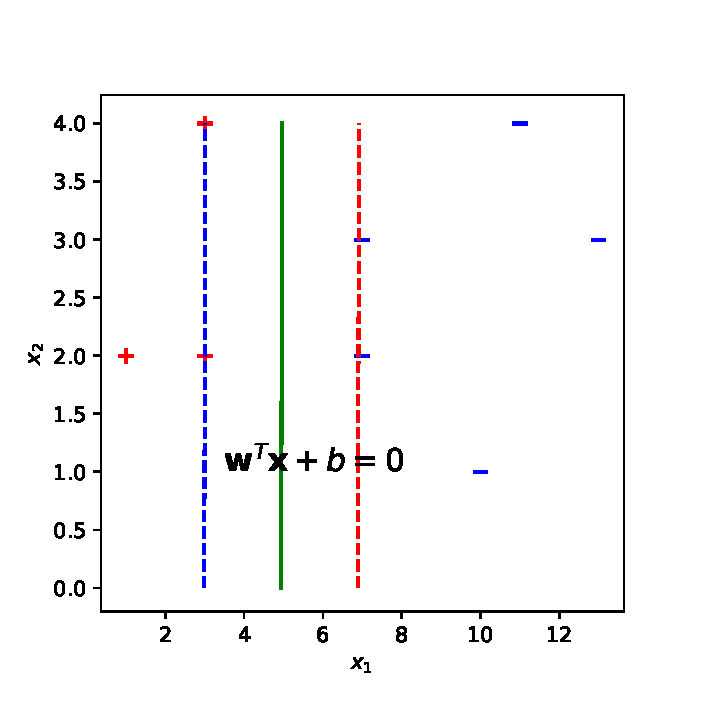
\includegraphics[width = 0.7\columnwidth]{pic-ex}
			}
		\end{minipage}
		\begin{minipage}[b]{0.48\textwidth}
			\centering
			\subfigure[$D=0.5$]{
				Here could be a graph.
			}
		\end{minipage}
		\DeclareGraphicsExtensions.
		\caption{Test graphs.}
		\label{fig:ex1:resD}
	\end{figure}

  \begin{theorem}[example]
    \vspace{0.5em}
    check the theorem.
  \end{theorem}

	\qED
	
\end{exercise}

\begin{solution}[proof]
  
Test subequations:

\begin{subequations}
    \renewcommand{\theequation}
    {\theparentequation-\arabic{equation}}
    \begin{align}
    \frac{\partial \mathcal{L}(\mathbf{w},~b)}{\partial \mathbf{w}} &= \mathbf{w} + C \sum\limits_i\frac{\partial \ell_i}{\partial \mathbf{w}}, \label{fml:ex1:partialW}\\
    \frac{\partial \mathcal{L}(\mathbf{w},~b)}{\partial b} &= C \sum\limits_i\frac{\partial \ell_i}{\partial b}, \label{fml:ex1:partialb}
    \end{align}
\end{subequations}
    
Test codings:

\lstinputlisting[language=Python]{./codes/Test.py}

\end{solution}

%\phantomsection
%\addcontentsline{toc}{section}{\refname}
\bibliographystyle{IEEEtran}
% argument is your BibTeX string definitions and bibliography database(s)
\bibliography{bib/refex}

\end{document}